\documentclass[tikz,border=0pt]{standalone}
\usepackage{xcolor}
% Palette: Sam_Comm_final.png by eye, and the cast's own colours.
\definecolor{ink}{HTML}{3B2340}
\definecolor{sky}{HTML}{EFC46A}
\definecolor{skyhi}{HTML}{F5DA92}
\definecolor{skylow}{HTML}{E9B060}
\definecolor{cloud}{HTML}{F2D58A}
\definecolor{wallA}{HTML}{E88A73}
\definecolor{wallB}{HTML}{EE9F7E}
\definecolor{wallC}{HTML}{E47A7E}
\definecolor{wallD}{HTML}{F0B07E}
\definecolor{wallE}{HTML}{D9765F}
\definecolor{wallF}{HTML}{E99A8A}
\definecolor{greenA}{HTML}{8DBB7E}
\definecolor{greenB}{HTML}{6FA77A}
\definecolor{greenC}{HTML}{A9C97F}
\definecolor{greenD}{HTML}{5E9C6A}
\definecolor{window}{HTML}{F6E7A0}
\definecolor{windark}{HTML}{8C5A64}
\definecolor{metal}{HTML}{8D9A93}
\definecolor{metaldark}{HTML}{5E6B66}
\definecolor{wood}{HTML}{B9835A}
\definecolor{paving}{HTML}{E2BD8C}
\definecolor{ground}{HTML}{D3A77D}
\definecolor{stone}{HTML}{E7C9A0}
\definecolor{road}{HTML}{C9957A}
\definecolor{roadline}{HTML}{F3DFA8}
\definecolor{paper}{HTML}{F6E7C4}
\definecolor{paperdark}{HTML}{E3CC98}
\definecolor{cardboard}{HTML}{C9A06A}
\definecolor{cardboarddark}{HTML}{A47C4C}
\definecolor{cutedge}{HTML}{A8998A}
\definecolor{magenta}{HTML}{FF2E88}
\definecolor{cyan}{HTML}{13CFE3}
\definecolor{gold}{HTML}{FFB000}
\definecolor{trim}{HTML}{F26B38}
\definecolor{violet}{HTML}{7B2FF7}
\definecolor{skin}{HTML}{E8B07C}
\definecolor{skinB}{HTML}{C98B5E}
\definecolor{skinC}{HTML}{F2C9A0}
\definecolor{skinshade}{HTML}{D4956A}
\definecolor{eyewhite}{HTML}{FBF4E4}
\definecolor{mouth}{HTML}{5A2238}
\definecolor{teeth}{HTML}{FBF4E4}
\definecolor{blush}{HTML}{F08A8A}
\definecolor{hairdark}{HTML}{2A1E33}
\definecolor{leather}{HTML}{33293D}
\definecolor{leatherhi}{HTML}{54466A}
\definecolor{denim}{HTML}{46597A}
\definecolor{guitar}{HTML}{D2463C}
\definecolor{goldbelt}{HTML}{F2B53A}
\definecolor{golddark}{HTML}{C98A1E}
\definecolor{red}{HTML}{B3262E}
\definecolor{royal}{HTML}{5E3A87}
\definecolor{fur}{HTML}{C98A55}
\definecolor{furlight}{HTML}{EBC592}
\definecolor{bow}{HTML}{E2577A}
\definecolor{patch}{HTML}{6FA77A}
\definecolor{chef}{HTML}{F6EBD2}
\definecolor{chefdark}{HTML}{D9C7A0}
\definecolor{shirt}{HTML}{5FA8A0}
\definecolor{check}{HTML}{9AA3A0}
\definecolor{toast}{HTML}{E9B55E}
\definecolor{crust}{HTML}{A8693C}
\definecolor{butter}{HTML}{F7DE6A}
\definecolor{tux}{HTML}{2E2638}
\definecolor{tuxhi}{HTML}{4F4460}
\definecolor{shirtwhite}{HTML}{F8F0DE}
\definecolor{chrome}{HTML}{C9D3CF}
\definecolor{chromedark}{HTML}{7F8C88}
\definecolor{velvet}{HTML}{A8324A}
\definecolor{ermine}{HTML}{F7F0DF}
\definecolor{gown}{HTML}{5E9C6A}
\definecolor{hairq}{HTML}{CFC6D8}
\definecolor{jewelB}{HTML}{13A6C9}
\definecolor{car}{HTML}{4FA3A5}
\definecolor{cardark}{HTML}{2F7476}
\definecolor{tyre}{HTML}{3E3A46}
\definecolor{glass}{HTML}{A9D4CB}
\definecolor{lamp}{HTML}{FFE6A3}
\definecolor{smoke}{HTML}{E8D3AE}
\definecolor{shingle}{HTML}{C9604F}
\begin{document}
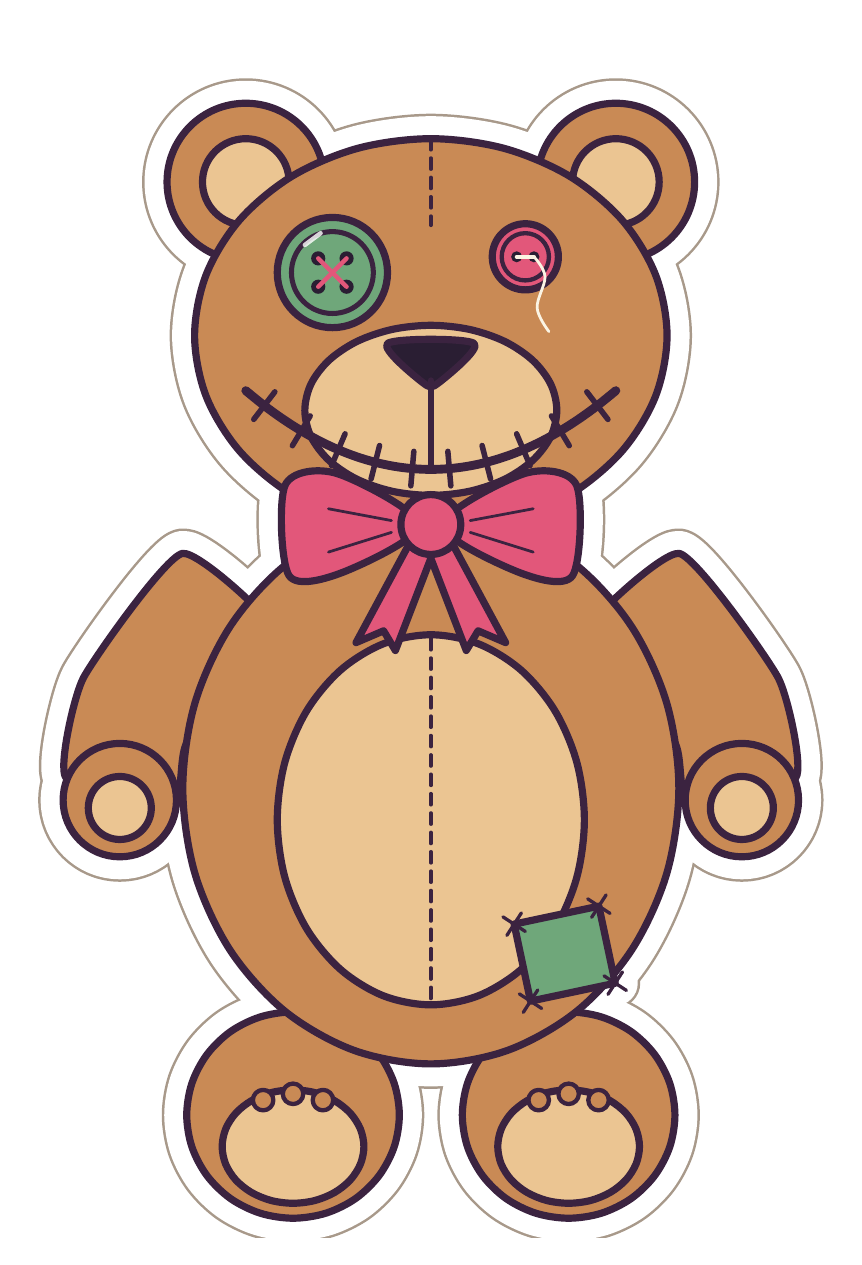
\begin{tikzpicture}
\clip (0,0) rectangle (10.24,15.36);
\filldraw[draw=cutedge, fill=cutedge, line width=18.057pt, line join=round] (2.77,13.4) circle (1);
\filldraw[draw=cutedge, fill=cutedge, line width=18.057pt, line join=round] (2.77,13.4) circle (0.55);
\filldraw[draw=cutedge, fill=cutedge, line width=18.057pt, line join=round] (7.47,13.4) circle (1);
\filldraw[draw=cutedge, fill=cutedge, line width=18.057pt, line join=round] (7.47,13.4) circle (0.55);
\filldraw[draw=cutedge, fill=cutedge, line width=18.057pt, line join=round] plot[smooth cycle, tension=0.3] coordinates {(3.273,7.517) (2.033,6.299) (1.856,5.563) (0.484,5.837) (0.707,7.101) (1.967,8.683)};
\filldraw[draw=cutedge, fill=cutedge, line width=18.057pt, line join=round] (1.17,5.55) circle (0.72);
\filldraw[draw=cutedge, fill=cutedge, line width=18.057pt, line join=round] (1.17,5.45) circle (0.4);
\filldraw[draw=cutedge, fill=cutedge, line width=18.057pt, line join=round] plot[smooth cycle, tension=0.3] coordinates {(8.273,8.683) (9.533,7.101) (9.756,5.837) (8.384,5.563) (8.207,6.299) (6.967,7.517)};
\filldraw[draw=cutedge, fill=cutedge, line width=18.057pt, line join=round] (9.07,5.55) circle (0.72);
\filldraw[draw=cutedge, fill=cutedge, line width=18.057pt, line join=round] (9.07,5.45) circle (0.4);
\filldraw[draw=cutedge, fill=cutedge, line width=18.057pt, line join=round] plot[smooth cycle, tension=0.55] coordinates {(4.72,1.55) (4.654,1.955) (4.462,2.32) (4.164,2.61) (3.787,2.796) (3.37,2.86) (2.953,2.796) (2.576,2.61) (2.278,2.32) (2.086,1.955) (2.02,1.55) (2.086,1.145) (2.278,0.78) (2.576,0.49) (2.953,0.304) (3.37,0.24) (3.787,0.304) (4.164,0.49) (4.462,0.78) (4.654,1.145)};
\filldraw[draw=cutedge, fill=cutedge, line width=18.057pt, line join=round] plot[smooth cycle, tension=0.55] coordinates {(8.22,1.55) (8.154,1.955) (7.962,2.32) (7.664,2.61) (7.287,2.796) (6.87,2.86) (6.453,2.796) (6.076,2.61) (5.778,2.32) (5.586,1.955) (5.52,1.55) (5.586,1.145) (5.778,0.78) (6.076,0.49) (6.453,0.304) (6.87,0.24) (7.287,0.304) (7.664,0.49) (7.962,0.78) (8.154,1.145)};
\filldraw[draw=cutedge, fill=cutedge, line width=18.057pt, line join=round] plot[smooth cycle, tension=0.55] coordinates {(8.27,5.7) (8.116,6.782) (7.668,7.757) (6.972,8.532) (6.093,9.029) (5.12,9.2) (4.147,9.029) (3.268,8.532) (2.572,7.757) (2.124,6.782) (1.97,5.7) (2.124,4.618) (2.572,3.643) (3.268,2.868) (4.147,2.371) (5.12,2.2) (6.093,2.371) (6.972,2.868) (7.668,3.643) (8.116,4.618)};
\filldraw[draw=cutedge, fill=cutedge, line width=18.057pt, line join=round] plot[smooth cycle, tension=0.55] coordinates {(7.07,5.3) (6.975,6.026) (6.698,6.681) (6.266,7.201) (5.723,7.535) (5.12,7.65) (4.517,7.535) (3.974,7.201) (3.542,6.681) (3.265,6.026) (3.17,5.3) (3.265,4.574) (3.542,3.919) (3.974,3.399) (4.517,3.065) (5.12,2.95) (5.723,3.065) (6.266,3.399) (6.698,3.919) (6.975,4.574)};
\filldraw[draw=cutedge, fill=cutedge, line width=18.057pt, line join=round] plot[smooth cycle, tension=0.55] coordinates {(4.27,1.15) (4.226,1.372) (4.098,1.573) (3.899,1.732) (3.648,1.835) (3.37,1.87) (3.092,1.835) (2.841,1.732) (2.642,1.573) (2.514,1.372) (2.47,1.15) (2.514,0.928) (2.642,0.727) (2.841,0.568) (3.092,0.465) (3.37,0.43) (3.648,0.465) (3.899,0.568) (4.098,0.727) (4.226,0.928)};
\filldraw[draw=cutedge, fill=cutedge, line width=18.057pt, line join=round] (2.99,1.74) circle (0.13);
\filldraw[draw=cutedge, fill=cutedge, line width=18.057pt, line join=round] (3.37,1.82) circle (0.13);
\filldraw[draw=cutedge, fill=cutedge, line width=18.057pt, line join=round] (3.75,1.74) circle (0.13);
\filldraw[draw=cutedge, fill=cutedge, line width=18.057pt, line join=round] plot[smooth cycle, tension=0.55] coordinates {(7.77,1.15) (7.726,1.372) (7.598,1.573) (7.399,1.732) (7.148,1.835) (6.87,1.87) (6.592,1.835) (6.341,1.732) (6.142,1.573) (6.014,1.372) (5.97,1.15) (6.014,0.928) (6.142,0.727) (6.341,0.568) (6.592,0.465) (6.87,0.43) (7.148,0.465) (7.399,0.568) (7.598,0.727) (7.726,0.928)};
\filldraw[draw=cutedge, fill=cutedge, line width=18.057pt, line join=round] (6.49,1.74) circle (0.13);
\filldraw[draw=cutedge, fill=cutedge, line width=18.057pt, line join=round] (6.87,1.82) circle (0.13);
\filldraw[draw=cutedge, fill=cutedge, line width=18.057pt, line join=round] (7.25,1.74) circle (0.13);
\filldraw[draw=cutedge, fill=cutedge, line width=18.057pt, line join=round] (6.386,2.997) -- (7.462,3.225) -- (7.254,4.203) -- (6.178,3.975) -- cycle;
\filldraw[draw=cutedge, fill=cutedge, line width=18.057pt, line join=round] plot[smooth cycle, tension=0.55] coordinates {(8.12,11.45) (7.973,12.223) (7.547,12.919) (6.883,13.473) (6.047,13.828) (5.12,13.95) (4.193,13.828) (3.357,13.473) (2.693,12.919) (2.267,12.223) (2.12,11.45) (2.267,10.677) (2.693,9.981) (3.357,9.427) (4.193,9.072) (5.12,8.95) (6.047,9.072) (6.883,9.427) (7.547,9.981) (7.973,10.677)};
\filldraw[draw=cutedge, fill=cutedge, line width=18.057pt, line join=round] plot[smooth cycle, tension=0.55] coordinates {(6.72,10.5) (6.642,10.834) (6.414,11.135) (6.06,11.374) (5.614,11.527) (5.12,11.58) (4.626,11.527) (4.18,11.374) (3.826,11.135) (3.598,10.834) (3.52,10.5) (3.598,10.166) (3.826,9.865) (4.18,9.626) (4.626,9.473) (5.12,9.42) (5.614,9.473) (6.06,9.626) (6.414,9.865) (6.642,10.166)};
\filldraw[draw=cutedge, fill=cutedge, line width=18.057pt, line join=round] plot[smooth cycle, tension=0.5] coordinates {(4.57,11.35) (5.67,11.35) (5.22,10.85) (5.02,10.85)};
\filldraw[draw=cutedge, fill=cutedge, line width=18.057pt, line join=round] (3.87,12.25) circle (0.7);
\filldraw[draw=cutedge, fill=cutedge, line width=18.057pt, line join=round] (3.87,12.25) circle (0.52);
\filldraw[draw=cutedge, fill=cutedge, line width=18.057pt, line join=round] (3.69,12.43) circle (0.09);
\filldraw[draw=cutedge, fill=cutedge, line width=18.057pt, line join=round] (4.05,12.43) circle (0.09);
\filldraw[draw=cutedge, fill=cutedge, line width=18.057pt, line join=round] (4.05,12.07) circle (0.09);
\filldraw[draw=cutedge, fill=cutedge, line width=18.057pt, line join=round] (3.69,12.07) circle (0.09);
\filldraw[draw=cutedge, fill=cutedge, line width=18.057pt, line join=round] (6.32,12.45) circle (0.42);
\filldraw[draw=cutedge, fill=cutedge, line width=18.057pt, line join=round] (6.32,12.45) circle (0.3);
\filldraw[draw=cutedge, fill=cutedge, line width=18.057pt, line join=round] (6.21,12.45) circle (0.07);
\filldraw[draw=cutedge, fill=cutedge, line width=18.057pt, line join=round] (6.43,12.45) circle (0.07);
\filldraw[draw=cutedge, fill=cutedge, line width=18.057pt, line join=round] plot[smooth cycle, tension=0.5] coordinates {(4.97,9.05) (3.92,9.7) (3.27,9.55) (3.32,8.4) (4.02,8.45)};
\filldraw[draw=cutedge, fill=cutedge, line width=18.057pt, line join=round] plot[smooth cycle, tension=0.5] coordinates {(5.27,9.05) (6.32,9.7) (6.97,9.55) (6.92,8.4) (6.22,8.45)};
\filldraw[draw=cutedge, fill=cutedge, line width=18.057pt, line join=round] (4.87,8.85) -- (4.17,7.55) -- (4.52,7.7) -- (4.67,7.45) -- (5.17,8.75) -- cycle;
\filldraw[draw=cutedge, fill=cutedge, line width=18.057pt, line join=round] (5.37,8.85) -- (6.07,7.55) -- (5.72,7.7) -- (5.57,7.45) -- (5.07,8.75) -- cycle;
\filldraw[draw=cutedge, fill=cutedge, line width=18.057pt, line join=round] (5.12,9.05) circle (0.38);
\filldraw[draw=white, fill=white, line width=16.257pt, line join=round] (2.77,13.4) circle (1);
\filldraw[draw=white, fill=white, line width=16.257pt, line join=round] (2.77,13.4) circle (0.55);
\filldraw[draw=white, fill=white, line width=16.257pt, line join=round] (7.47,13.4) circle (1);
\filldraw[draw=white, fill=white, line width=16.257pt, line join=round] (7.47,13.4) circle (0.55);
\filldraw[draw=white, fill=white, line width=16.257pt, line join=round] plot[smooth cycle, tension=0.3] coordinates {(3.273,7.517) (2.033,6.299) (1.856,5.563) (0.484,5.837) (0.707,7.101) (1.967,8.683)};
\filldraw[draw=white, fill=white, line width=16.257pt, line join=round] (1.17,5.55) circle (0.72);
\filldraw[draw=white, fill=white, line width=16.257pt, line join=round] (1.17,5.45) circle (0.4);
\filldraw[draw=white, fill=white, line width=16.257pt, line join=round] plot[smooth cycle, tension=0.3] coordinates {(8.273,8.683) (9.533,7.101) (9.756,5.837) (8.384,5.563) (8.207,6.299) (6.967,7.517)};
\filldraw[draw=white, fill=white, line width=16.257pt, line join=round] (9.07,5.55) circle (0.72);
\filldraw[draw=white, fill=white, line width=16.257pt, line join=round] (9.07,5.45) circle (0.4);
\filldraw[draw=white, fill=white, line width=16.257pt, line join=round] plot[smooth cycle, tension=0.55] coordinates {(4.72,1.55) (4.654,1.955) (4.462,2.32) (4.164,2.61) (3.787,2.796) (3.37,2.86) (2.953,2.796) (2.576,2.61) (2.278,2.32) (2.086,1.955) (2.02,1.55) (2.086,1.145) (2.278,0.78) (2.576,0.49) (2.953,0.304) (3.37,0.24) (3.787,0.304) (4.164,0.49) (4.462,0.78) (4.654,1.145)};
\filldraw[draw=white, fill=white, line width=16.257pt, line join=round] plot[smooth cycle, tension=0.55] coordinates {(8.22,1.55) (8.154,1.955) (7.962,2.32) (7.664,2.61) (7.287,2.796) (6.87,2.86) (6.453,2.796) (6.076,2.61) (5.778,2.32) (5.586,1.955) (5.52,1.55) (5.586,1.145) (5.778,0.78) (6.076,0.49) (6.453,0.304) (6.87,0.24) (7.287,0.304) (7.664,0.49) (7.962,0.78) (8.154,1.145)};
\filldraw[draw=white, fill=white, line width=16.257pt, line join=round] plot[smooth cycle, tension=0.55] coordinates {(8.27,5.7) (8.116,6.782) (7.668,7.757) (6.972,8.532) (6.093,9.029) (5.12,9.2) (4.147,9.029) (3.268,8.532) (2.572,7.757) (2.124,6.782) (1.97,5.7) (2.124,4.618) (2.572,3.643) (3.268,2.868) (4.147,2.371) (5.12,2.2) (6.093,2.371) (6.972,2.868) (7.668,3.643) (8.116,4.618)};
\filldraw[draw=white, fill=white, line width=16.257pt, line join=round] plot[smooth cycle, tension=0.55] coordinates {(7.07,5.3) (6.975,6.026) (6.698,6.681) (6.266,7.201) (5.723,7.535) (5.12,7.65) (4.517,7.535) (3.974,7.201) (3.542,6.681) (3.265,6.026) (3.17,5.3) (3.265,4.574) (3.542,3.919) (3.974,3.399) (4.517,3.065) (5.12,2.95) (5.723,3.065) (6.266,3.399) (6.698,3.919) (6.975,4.574)};
\filldraw[draw=white, fill=white, line width=16.257pt, line join=round] plot[smooth cycle, tension=0.55] coordinates {(4.27,1.15) (4.226,1.372) (4.098,1.573) (3.899,1.732) (3.648,1.835) (3.37,1.87) (3.092,1.835) (2.841,1.732) (2.642,1.573) (2.514,1.372) (2.47,1.15) (2.514,0.928) (2.642,0.727) (2.841,0.568) (3.092,0.465) (3.37,0.43) (3.648,0.465) (3.899,0.568) (4.098,0.727) (4.226,0.928)};
\filldraw[draw=white, fill=white, line width=16.257pt, line join=round] (2.99,1.74) circle (0.13);
\filldraw[draw=white, fill=white, line width=16.257pt, line join=round] (3.37,1.82) circle (0.13);
\filldraw[draw=white, fill=white, line width=16.257pt, line join=round] (3.75,1.74) circle (0.13);
\filldraw[draw=white, fill=white, line width=16.257pt, line join=round] plot[smooth cycle, tension=0.55] coordinates {(7.77,1.15) (7.726,1.372) (7.598,1.573) (7.399,1.732) (7.148,1.835) (6.87,1.87) (6.592,1.835) (6.341,1.732) (6.142,1.573) (6.014,1.372) (5.97,1.15) (6.014,0.928) (6.142,0.727) (6.341,0.568) (6.592,0.465) (6.87,0.43) (7.148,0.465) (7.399,0.568) (7.598,0.727) (7.726,0.928)};
\filldraw[draw=white, fill=white, line width=16.257pt, line join=round] (6.49,1.74) circle (0.13);
\filldraw[draw=white, fill=white, line width=16.257pt, line join=round] (6.87,1.82) circle (0.13);
\filldraw[draw=white, fill=white, line width=16.257pt, line join=round] (7.25,1.74) circle (0.13);
\filldraw[draw=white, fill=white, line width=16.257pt, line join=round] (6.386,2.997) -- (7.462,3.225) -- (7.254,4.203) -- (6.178,3.975) -- cycle;
\filldraw[draw=white, fill=white, line width=16.257pt, line join=round] plot[smooth cycle, tension=0.55] coordinates {(8.12,11.45) (7.973,12.223) (7.547,12.919) (6.883,13.473) (6.047,13.828) (5.12,13.95) (4.193,13.828) (3.357,13.473) (2.693,12.919) (2.267,12.223) (2.12,11.45) (2.267,10.677) (2.693,9.981) (3.357,9.427) (4.193,9.072) (5.12,8.95) (6.047,9.072) (6.883,9.427) (7.547,9.981) (7.973,10.677)};
\filldraw[draw=white, fill=white, line width=16.257pt, line join=round] plot[smooth cycle, tension=0.55] coordinates {(6.72,10.5) (6.642,10.834) (6.414,11.135) (6.06,11.374) (5.614,11.527) (5.12,11.58) (4.626,11.527) (4.18,11.374) (3.826,11.135) (3.598,10.834) (3.52,10.5) (3.598,10.166) (3.826,9.865) (4.18,9.626) (4.626,9.473) (5.12,9.42) (5.614,9.473) (6.06,9.626) (6.414,9.865) (6.642,10.166)};
\filldraw[draw=white, fill=white, line width=16.257pt, line join=round] plot[smooth cycle, tension=0.5] coordinates {(4.57,11.35) (5.67,11.35) (5.22,10.85) (5.02,10.85)};
\filldraw[draw=white, fill=white, line width=16.257pt, line join=round] (3.87,12.25) circle (0.7);
\filldraw[draw=white, fill=white, line width=16.257pt, line join=round] (3.87,12.25) circle (0.52);
\filldraw[draw=white, fill=white, line width=16.257pt, line join=round] (3.69,12.43) circle (0.09);
\filldraw[draw=white, fill=white, line width=16.257pt, line join=round] (4.05,12.43) circle (0.09);
\filldraw[draw=white, fill=white, line width=16.257pt, line join=round] (4.05,12.07) circle (0.09);
\filldraw[draw=white, fill=white, line width=16.257pt, line join=round] (3.69,12.07) circle (0.09);
\filldraw[draw=white, fill=white, line width=16.257pt, line join=round] (6.32,12.45) circle (0.42);
\filldraw[draw=white, fill=white, line width=16.257pt, line join=round] (6.32,12.45) circle (0.3);
\filldraw[draw=white, fill=white, line width=16.257pt, line join=round] (6.21,12.45) circle (0.07);
\filldraw[draw=white, fill=white, line width=16.257pt, line join=round] (6.43,12.45) circle (0.07);
\filldraw[draw=white, fill=white, line width=16.257pt, line join=round] plot[smooth cycle, tension=0.5] coordinates {(4.97,9.05) (3.92,9.7) (3.27,9.55) (3.32,8.4) (4.02,8.45)};
\filldraw[draw=white, fill=white, line width=16.257pt, line join=round] plot[smooth cycle, tension=0.5] coordinates {(5.27,9.05) (6.32,9.7) (6.97,9.55) (6.92,8.4) (6.22,8.45)};
\filldraw[draw=white, fill=white, line width=16.257pt, line join=round] (4.87,8.85) -- (4.17,7.55) -- (4.52,7.7) -- (4.67,7.45) -- (5.17,8.75) -- cycle;
\filldraw[draw=white, fill=white, line width=16.257pt, line join=round] (5.37,8.85) -- (6.07,7.55) -- (5.72,7.7) -- (5.57,7.45) -- (5.07,8.75) -- cycle;
\filldraw[draw=white, fill=white, line width=16.257pt, line join=round] (5.12,9.05) circle (0.38);
\filldraw[draw=ink, line width=2.6pt, line join=round, fill=fur] (2.77,13.4) circle (1);
\filldraw[draw=ink, line width=2.6pt, line join=round, fill=furlight] (2.77,13.4) circle (0.55);
\filldraw[draw=ink, line width=2.6pt, line join=round, fill=fur] (7.47,13.4) circle (1);
\filldraw[draw=ink, line width=2.6pt, line join=round, fill=furlight] (7.47,13.4) circle (0.55);
\filldraw[draw=ink, line width=2.6pt, line join=round, fill=fur] plot[smooth cycle, tension=0.3] coordinates {(3.273,7.517) (2.033,6.299) (1.856,5.563) (0.484,5.837) (0.707,7.101) (1.967,8.683)};
\filldraw[draw=ink, line width=2.6pt, line join=round, fill=fur] (1.17,5.55) circle (0.72);
\filldraw[draw=ink, line width=2.6pt, line join=round, fill=furlight] (1.17,5.45) circle (0.4);
\filldraw[draw=ink, line width=2.6pt, line join=round, fill=fur] plot[smooth cycle, tension=0.3] coordinates {(8.273,8.683) (9.533,7.101) (9.756,5.837) (8.384,5.563) (8.207,6.299) (6.967,7.517)};
\filldraw[draw=ink, line width=2.6pt, line join=round, fill=fur] (9.07,5.55) circle (0.72);
\filldraw[draw=ink, line width=2.6pt, line join=round, fill=furlight] (9.07,5.45) circle (0.4);
\filldraw[draw=ink, line width=2.6pt, line join=round, fill=fur] plot[smooth cycle, tension=0.55] coordinates {(4.72,1.55) (4.654,1.955) (4.462,2.32) (4.164,2.61) (3.787,2.796) (3.37,2.86) (2.953,2.796) (2.576,2.61) (2.278,2.32) (2.086,1.955) (2.02,1.55) (2.086,1.145) (2.278,0.78) (2.576,0.49) (2.953,0.304) (3.37,0.24) (3.787,0.304) (4.164,0.49) (4.462,0.78) (4.654,1.145)};
\filldraw[draw=ink, line width=2.6pt, line join=round, fill=fur] plot[smooth cycle, tension=0.55] coordinates {(8.22,1.55) (8.154,1.955) (7.962,2.32) (7.664,2.61) (7.287,2.796) (6.87,2.86) (6.453,2.796) (6.076,2.61) (5.778,2.32) (5.586,1.955) (5.52,1.55) (5.586,1.145) (5.778,0.78) (6.076,0.49) (6.453,0.304) (6.87,0.24) (7.287,0.304) (7.664,0.49) (7.962,0.78) (8.154,1.145)};
\filldraw[draw=ink, line width=2.6pt, line join=round, fill=fur] plot[smooth cycle, tension=0.55] coordinates {(8.27,5.7) (8.116,6.782) (7.668,7.757) (6.972,8.532) (6.093,9.029) (5.12,9.2) (4.147,9.029) (3.268,8.532) (2.572,7.757) (2.124,6.782) (1.97,5.7) (2.124,4.618) (2.572,3.643) (3.268,2.868) (4.147,2.371) (5.12,2.2) (6.093,2.371) (6.972,2.868) (7.668,3.643) (8.116,4.618)};
\filldraw[draw=ink, line width=2.6pt, line join=round, fill=furlight] plot[smooth cycle, tension=0.55] coordinates {(7.07,5.3) (6.975,6.026) (6.698,6.681) (6.266,7.201) (5.723,7.535) (5.12,7.65) (4.517,7.535) (3.974,7.201) (3.542,6.681) (3.265,6.026) (3.17,5.3) (3.265,4.574) (3.542,3.919) (3.974,3.399) (4.517,3.065) (5.12,2.95) (5.723,3.065) (6.266,3.399) (6.698,3.919) (6.975,4.574)};
\draw[ink, line width=1.3pt, line cap=round, line join=round, dash pattern=on 4pt off 3pt] (5.12,7.6) -- (5.12,3);
\filldraw[draw=ink, line width=2.6pt, line join=round, fill=furlight] plot[smooth cycle, tension=0.55] coordinates {(4.27,1.15) (4.226,1.372) (4.098,1.573) (3.899,1.732) (3.648,1.835) (3.37,1.87) (3.092,1.835) (2.841,1.732) (2.642,1.573) (2.514,1.372) (2.47,1.15) (2.514,0.928) (2.642,0.727) (2.841,0.568) (3.092,0.465) (3.37,0.43) (3.648,0.465) (3.899,0.568) (4.098,0.727) (4.226,0.928)};
\filldraw[draw=ink, line width=1.56pt, line join=round, fill=fur] (2.99,1.74) circle (0.13);
\filldraw[draw=ink, line width=1.56pt, line join=round, fill=fur] (3.37,1.82) circle (0.13);
\filldraw[draw=ink, line width=1.56pt, line join=round, fill=fur] (3.75,1.74) circle (0.13);
\filldraw[draw=ink, line width=2.6pt, line join=round, fill=furlight] plot[smooth cycle, tension=0.55] coordinates {(7.77,1.15) (7.726,1.372) (7.598,1.573) (7.399,1.732) (7.148,1.835) (6.87,1.87) (6.592,1.835) (6.341,1.732) (6.142,1.573) (6.014,1.372) (5.97,1.15) (6.014,0.928) (6.142,0.727) (6.341,0.568) (6.592,0.465) (6.87,0.43) (7.148,0.465) (7.399,0.568) (7.598,0.727) (7.726,0.928)};
\filldraw[draw=ink, line width=1.56pt, line join=round, fill=fur] (6.49,1.74) circle (0.13);
\filldraw[draw=ink, line width=1.56pt, line join=round, fill=fur] (6.87,1.82) circle (0.13);
\filldraw[draw=ink, line width=1.56pt, line join=round, fill=fur] (7.25,1.74) circle (0.13);
\filldraw[draw=ink, line width=2.6pt, line join=round, fill=patch] (6.386,2.997) -- (7.462,3.225) -- (7.254,4.203) -- (6.178,3.975) -- cycle;
\draw[ink, line width=1.2pt, line cap=round, line join=round] (6.294,2.854) -- (6.478,3.139);
\draw[ink, line width=1.2pt, line cap=round, line join=round] (6.244,3.089) -- (6.528,2.904);
\draw[ink, line width=1.2pt, line cap=round, line join=round] (7.37,3.083) -- (7.554,3.368);
\draw[ink, line width=1.2pt, line cap=round, line join=round] (7.32,3.318) -- (7.604,3.133);
\draw[ink, line width=1.2pt, line cap=round, line join=round] (7.162,4.061) -- (7.346,4.346);
\draw[ink, line width=1.2pt, line cap=round, line join=round] (7.112,4.296) -- (7.396,4.111);
\draw[ink, line width=1.2pt, line cap=round, line join=round] (6.086,3.832) -- (6.27,4.117);
\draw[ink, line width=1.2pt, line cap=round, line join=round] (6.036,4.067) -- (6.32,3.882);
\filldraw[draw=ink, line width=2.6pt, line join=round, fill=fur] plot[smooth cycle, tension=0.55] coordinates {(8.12,11.45) (7.973,12.223) (7.547,12.919) (6.883,13.473) (6.047,13.828) (5.12,13.95) (4.193,13.828) (3.357,13.473) (2.693,12.919) (2.267,12.223) (2.12,11.45) (2.267,10.677) (2.693,9.981) (3.357,9.427) (4.193,9.072) (5.12,8.95) (6.047,9.072) (6.883,9.427) (7.547,9.981) (7.973,10.677)};
\draw[ink, line width=1.3pt, line cap=round, line join=round, dash pattern=on 4pt off 3pt] (5.12,13.95) -- (5.12,12.85);
\filldraw[draw=ink, line width=2.6pt, line join=round, fill=furlight] plot[smooth cycle, tension=0.55] coordinates {(6.72,10.5) (6.642,10.834) (6.414,11.135) (6.06,11.374) (5.614,11.527) (5.12,11.58) (4.626,11.527) (4.18,11.374) (3.826,11.135) (3.598,10.834) (3.52,10.5) (3.598,10.166) (3.826,9.865) (4.18,9.626) (4.626,9.473) (5.12,9.42) (5.614,9.473) (6.06,9.626) (6.414,9.865) (6.642,10.166)};
\filldraw[draw=ink, line width=2.6pt, line join=round, fill=hairdark] plot[smooth cycle, tension=0.5] coordinates {(4.57,11.35) (5.67,11.35) (5.22,10.85) (5.02,10.85)};
\draw[ink, line width=2.2pt, line cap=round, line join=round] (5.12,10.88) -- (5.12,9.78);
\draw[ink, line width=3.2pt, line cap=round, line join=round] plot[smooth, tension=0.6] coordinates {(2.77,10.75) (3.005,10.56) (3.24,10.39) (3.475,10.24) (3.71,10.11) (3.945,10) (4.18,9.91) (4.415,9.84) (4.65,9.79) (4.885,9.76) (5.12,9.75) (5.355,9.76) (5.59,9.79) (5.825,9.84) (6.06,9.91) (6.295,10) (6.53,10.11) (6.765,10.24) (7,10.39) (7.235,10.56) (7.47,10.75)};
\draw[ink, line width=2pt, line cap=round, line join=round] (2.871,10.385) -- (3.139,10.735);
\draw[ink, line width=2pt, line cap=round, line join=round] (3.362,10.051) -- (3.588,10.429);
\draw[ink, line width=2pt, line cap=round, line join=round] (3.859,9.798) -- (4.031,10.202);
\draw[ink, line width=2pt, line cap=round, line join=round] (4.361,9.627) -- (4.469,10.053);
\draw[ink, line width=2pt, line cap=round, line join=round] (4.866,9.541) -- (4.904,9.979);
\draw[ink, line width=2pt, line cap=round, line join=round] (5.374,9.541) -- (5.336,9.979);
\draw[ink, line width=2pt, line cap=round, line join=round] (5.879,9.627) -- (5.771,10.053);
\draw[ink, line width=2pt, line cap=round, line join=round] (6.381,9.798) -- (6.209,10.202);
\draw[ink, line width=2pt, line cap=round, line join=round] (6.878,10.051) -- (6.652,10.429);
\draw[ink, line width=2pt, line cap=round, line join=round] (7.369,10.385) -- (7.101,10.735);
\filldraw[draw=ink, line width=2.6pt, line join=round, fill=patch] (3.87,12.25) circle (0.7);
\filldraw[draw=ink, line width=1.82pt, line join=round, fill=patch] (3.87,12.25) circle (0.52);
\fill[hairdark] (3.69,12.43) circle (0.09);
\fill[hairdark] (4.05,12.43) circle (0.09);
\fill[hairdark] (4.05,12.07) circle (0.09);
\fill[hairdark] (3.69,12.07) circle (0.09);
\draw[bow, line width=1.6pt, line cap=round, line join=round] (3.69,12.43) -- (4.05,12.07);
\draw[bow, line width=1.6pt, line cap=round, line join=round] (4.05,12.43) -- (3.69,12.07);
\draw[white, line width=1.6pt, line cap=round, line join=round, opacity=0.8] (3.52,12.6) -- (3.72,12.75);
\filldraw[draw=ink, line width=2.6pt, line join=round, fill=bow] (6.32,12.45) circle (0.42);
\filldraw[draw=ink, line width=1.56pt, line join=round, fill=bow] (6.32,12.45) circle (0.3);
\fill[hairdark] (6.21,12.45) circle (0.07);
\fill[hairdark] (6.43,12.45) circle (0.07);
\draw[eyewhite, line width=1.4pt, line cap=round, line join=round] (6.21,12.45) -- (6.43,12.45);
\draw[eyewhite, line width=1pt, line cap=round, line join=round] plot[smooth, tension=0.6] coordinates {(6.43,12.45) (6.57,12.2) (6.47,11.8) (6.62,11.5)};
\filldraw[draw=ink, line width=2.6pt, line join=round, fill=bow] plot[smooth cycle, tension=0.5] coordinates {(4.97,9.05) (3.92,9.7) (3.27,9.55) (3.32,8.4) (4.02,8.45)};
\filldraw[draw=ink, line width=2.6pt, line join=round, fill=bow] plot[smooth cycle, tension=0.5] coordinates {(5.27,9.05) (6.32,9.7) (6.97,9.55) (6.92,8.4) (6.22,8.45)};
\filldraw[draw=ink, line width=2.6pt, line join=round, fill=bow] (4.87,8.85) -- (4.17,7.55) -- (4.52,7.7) -- (4.67,7.45) -- (5.17,8.75) -- cycle;
\filldraw[draw=ink, line width=2.6pt, line join=round, fill=bow] (5.37,8.85) -- (6.07,7.55) -- (5.72,7.7) -- (5.57,7.45) -- (5.07,8.75) -- cycle;
\filldraw[draw=ink, line width=2.6pt, line join=round, fill=bow] (5.12,9.05) circle (0.38);
\draw[ink, line width=1pt, line cap=round, line join=round] (4.62,9.1) -- (3.82,9.25);
\draw[ink, line width=1pt, line cap=round, line join=round] (4.62,8.95) -- (3.82,8.7);
\draw[ink, line width=1pt, line cap=round, line join=round] (5.62,9.1) -- (6.42,9.25);
\draw[ink, line width=1pt, line cap=round, line join=round] (5.62,8.95) -- (6.42,8.7);
\end{tikzpicture}
\end{document}
